\section{Cache Optimizations}
\label{sec:cache_opt}

Our cache optimizations for DNN training are based on the sparse nature of the performance critical data (e.g., activations, errors, etc.).  Our approach improves cache performance through a compact representation of cache lines containing only zeroes (a.k.a. \emph{zero cache lines}) in the caches, which helps to avoid  the normal bandwidth and storage costs of zero cache lines. These optimizations enable efficient scaling of model size and training threads.  

Managing zero data at cache line granularity makes it possible to realize our optimizations through simple and efficient extensions of existing memory systems.  Our current design comprises of mechanisms for achieving the following: (i) compact representation of zero cache lines, (ii) a decoupled cache hierarchy for zero cache lines, and (iii) tracking zero cache lines in the memory system.  We describe these mechanims in the rest of this section.

\subsection{Zero Cache Line Representation}

Our compact representation exploits the fact that the data bytes of a zero cache line are not required to represent the line in cache, the cache tag is sufficient for this purpose. Also, it is not neccesary to transfer the data bytes of a zero cache line across the caches since they can be synthesized in the processor (read) or main memory (on a writeback) as appropriate.  However, in event of a cache hit, we must quickly determine whether it is a zero cache line that is referenced so that the appropriate data transfer is done promptly. We consider two alternatives for handling this: (i) an extra bit in the cache tags to identify zero cache lines, or (ii) a decoupled hierarchy of cache tags for zero cache lines.  Although the first option avoids the extra cost of zero cache line tags, the data bytes space of zero cache lines are unused.  To avoid this waste, we adopt the second option in our current work. 

\begin{figure}[!t]
\centering
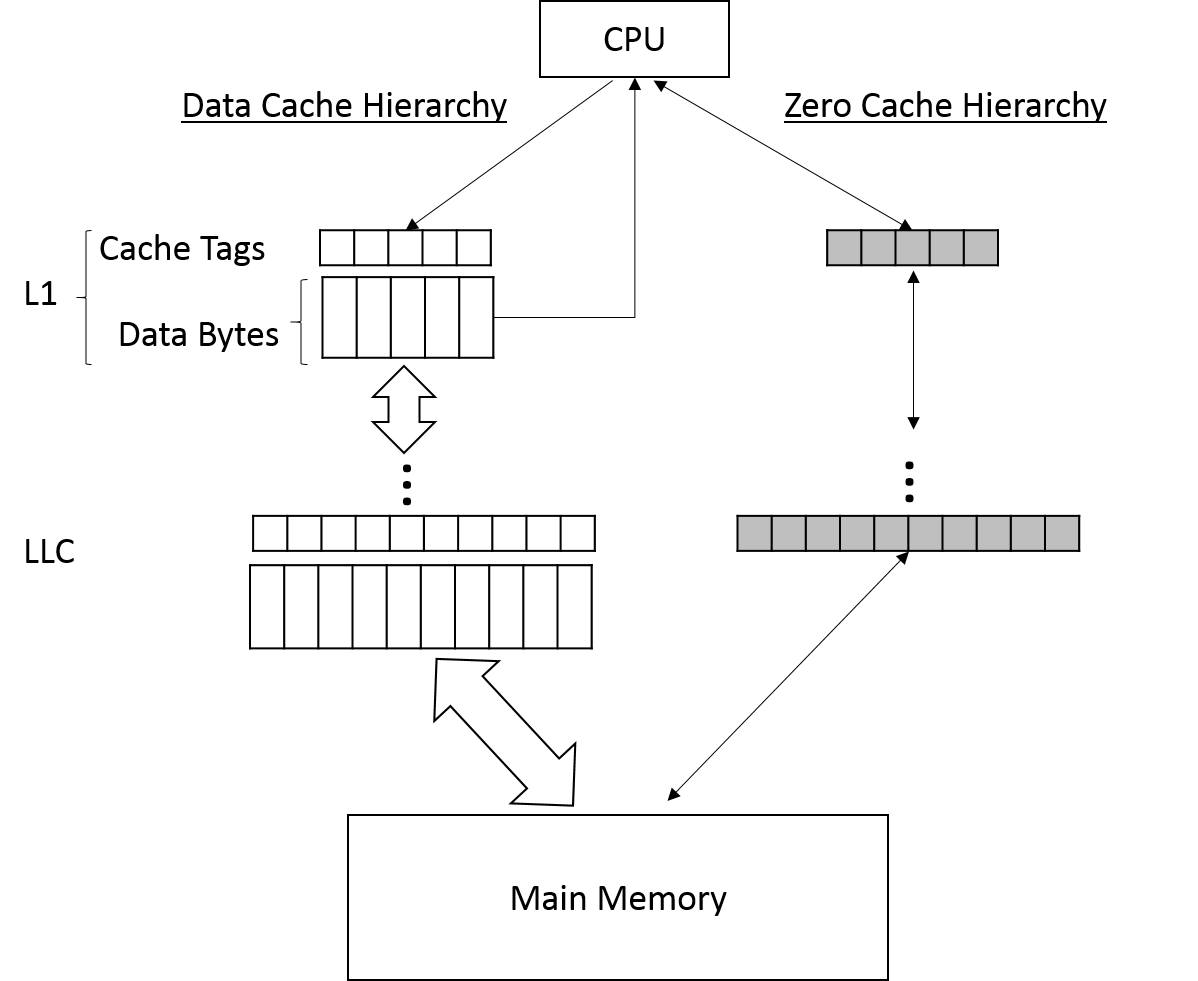
\includegraphics[width=2.4in]{Figures/zero_cache_hierarchy.png}
\caption{A Memory System with Zero Cache Hierarchy.}
\label{fig:zero_cache_hierarchy}
\end{figure}

\subsection{Hierarchy of Zero Cache Lines}

Figure~\ref{fig:zero_cache_hierarchy} illustrates a memory system that is augmented with a cache hierarchy for zero cache lines, which we call the \emph{zero cache} hierarchy. The zero cache hierarchy is a multi-level structure with caches (a.k.a., \emph{zero caches}) containing tags but no data bytes.  Since zero cache lines are not maintained in the conventional data caches, both cache hierarchies are mutually exclusive. The zero cache hierarchy and the data cache hierarchy have the same number of levels, and can additionally share other properties, such as number of entries, ways, associativity, replacement policies, etc.  The coherence of zero caches is maintained across cores using the same protocol as the data caches. 

Data access requests from the processor are satisfied by accessing the two cache hierarchies in parallel to avoid introducing extra latency. Figure~\ref{fig:cache_access_flowchart} shows the processing of a read request by the $N$th level caches.  The request is processed in parallel by the data  and zero caches, and forwarded to the next level if it is a miss in both.  If the request is a hit in either cache, then the appropriate response is sent to the processor or lower levels of the cache hierarchy.   The data cache responds, in the normal fashion, with the requested data bytes (or cache line), while the zero cache signals a zero cache line hit response. 

\begin{figure}[!t]
\centering
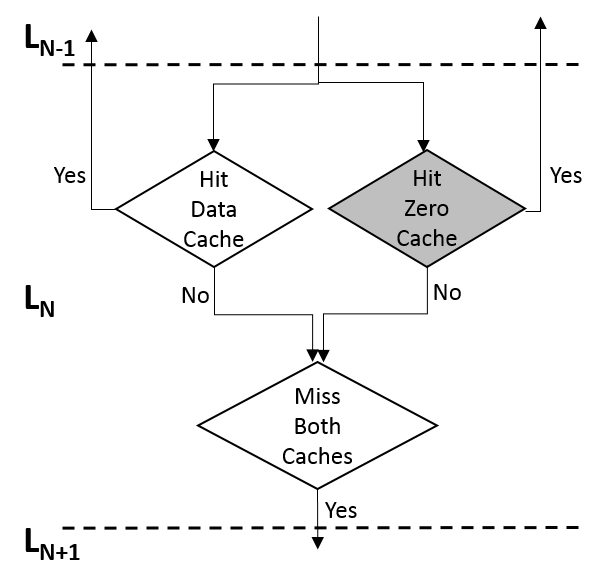
\includegraphics[ height=2in]{Figures/cache_access_flowchart.png}
\caption{Processing read requests with zero caches.}
\label{fig:cache_access_flowchart}
\end{figure}

\subsection{Tracking Zero Cache Lines}

We track zero cache lines in the memory system, as they originate from main memory and are transferred through the zero cache hierarchy. We describe how to detect transitions of cache lines from zero to non-zero status based on processor writes, and describe a protocol for migrating cache lines between the data caches and zero caches. 

